\documentclass[notitlepage,letterpaper,pdftex,12pt,final]{article}
%\documentclass[notitlepage,letterpaper,pdftex,12pt,draft]{article}
% article < report < book ; preable material follows
%
% This file is mostly boilerplate that you can copy and tweak.
% The true material is in included files.  ../common should hold
% things that more than one document might need.  The Makefiles
% should likewise be mostly boilerplate with minor tweaks.
%

% (un)comment to (see)hide full paths to files actually used
% however, you'll need to override the TEXOPT= setting to batchmode
% made in the Makefile.
\listfiles

\addtolength\textwidth{1.7in}
\addtolength\oddsidemargin{-0.95in}
\addtolength\evensidemargin{-0.95in}
\addtolength\marginparwidth{-0.95in}
\typeout{textwidth is \the\textwidth}

% useful to block out portions of text
\usepackage{ifthen}
% to allow defining our own colors
\usepackage[dvipsnames]{xcolor}
% makes hyperlinks work
\usepackage{hyperref}
\hypersetup{colorlinks=true,linkcolor=darkblue,citecolor=darkgreen}
% for figures; insert [draft] before {...} not to see imgs
\usepackage{graphicx}
% for small figures surrounded by text
\usepackage{wrapfig}
% for control over headers and footers
\usepackage{fancyhdr}
\pagestyle{fancy}
\fancyhf{}
% for handling acronyms
\usepackage[printonlyused]{acronym}

\usepackage{array}
%\usepackage{multirow}

% for bibliographies if needed
\usepackage[utf8]{inputenc}
\usepackage[english]{babel}
\usepackage[backend=biber,style=numeric,sorting=none]{biblatex}
\addbibresource{hops.bib}
% context-sensitive quotes
\usepackage{csquotes}
% underline for emphasis: \uline etc
\usepackage{ulem}
% for generating outlines
\usepackage{outlines}
\usepackage{enumitem}

% for bold math
\usepackage{bm}
% for serious math which we may have in a few places (eventually)
\usepackage{amsmath}
% equations include section number
\numberwithin{equation}{section}

% for marginal notations concerning geodesy
\usepackage{marginnote}

% to go back to default after \ragged commmands
\usepackage{ragged2e}

\usepackage[font=small]{caption}

% see common/shortcuts.tex for what is defined in this file
%
% a file of commands to save typing
%

% commonly used things
\newcommand{\eg}{\textit{e.g.}}
\newcommand{\EG}{\textit{E.g.}}
\newcommand{\ie}{\textit{i.e.}}
\newcommand{\IE}{\textit{I.e.}}
\newcommand{\etc}{\textit{\&c.}}
\newcommand{\Sec}{Section}
\newcommand{\Fig}{Figure}
\newcommand{\Tab}{Table}
\newcommand{\App}{Appendix}

% for a work in progress:
\newcommand{\FIX}[1][fixme]{{\color{red}#1}}
\newcommand{\TBC}{{\color{red}TBC}}
\newcommand{\TBD}{{\color{red}TBD}}
\newcommand{\TBR}{{\color{red}TBR}}
\newcommand{\FIXME}[1][]{{\color{red}FIXME -- #1}}

% specific to this project
\newcommand{\MHO}{MIT-HOPS}
\newcommand{\HOPS}{HOPS}

% standard colors
\definecolor{darkblue}{rgb}{0,0,.5}
\definecolor{darkgreen}{rgb}{0,.5,0}
\definecolor{darkred}{rgb}{.5,0,0}
\definecolor{violet}{rgb}{.4,0.,.7}

% for coping with geodetic things
\newboolean{geos}
\setboolean{geos}{true}% or false to hide geodetic marginal notations
%
\definecolor{boxfrcolor}{rgb}{.50,.20,.00}
\definecolor{boxbgcolor}{rgb}{0.9,.98,.98}
\definecolor{boxfgcolor}{rgb}{0.4,0.0,0.0}
% \geomargin{footnote comment}
% \geomargin[{\color{..}box note}]{footnote comment}
\newcommand{\geobox}[1]%
{{\parbox{10mm}{\small\textit{\fcolorbox{boxfrcolor}{boxbgcolor}{#1}}}}}
\newcommand{\geomargin}[2][{\color{boxfgcolor}geodesy}]%
{\ifthenelse{\boolean{geos}}{% if:
\marginnote{\protect\geobox{#1}}\footnote{#2}}{% else: show nothing
}}

% for itemizing requirements
\newcounter{req}
\newcommand{\reqid}[1]{\item[\refstepcounter{req}#1-\thereq]}

%
% eof
%

\setboolean{geos}{true}% or false to hide geodetic marginal notations

% control options
\newboolean{skipappendix}
\setboolean{skipappendix}{false}

% at some point this gets frozen
\newcommand{\recdate}{\today}

\begin{document}
\DeclareGraphicsExtensions{.png, .jpg, .pdf}
% best to put figures in subdirs
%\graphicspath{{figs/}{scans/}}

% for subsequent pages
\setlength\headheight{15pt}
\fancyhead[L]{HOPS}
\fancyhead[C]{}
\fancyhead[R]{Requirements}
\fancyfoot[R]{Page \thepage\ of\ \pageref{page:LastPage}}
\fancyfoot[L]{\recdate}

\title{ngEHT Development Plan for a new HOPS}

\author{%
\LARGE John Barrett, Geoff Crew, Dan Hoak and Violet Pfeiffer \\
\Large MIT Haystack Observatory}
\date{Version 0.1, \recdate}
\maketitle
\normalsize

\renewcommand\abstractname{Executive Summary}
\abstract{%
\large
This document describes the plan for executing the HOPS MSRI refactoring.
We shall generally be following an agile development plan
which involves an iterative approach to the software development
once the basic infrastructure and design principal are settled.
There are also sections on other programmatic elements.
}

% \begingroup . . . \endgroup can be used to keep things together
% and/or an explicit page break and/or adjust spacing as needed so
% it looks presentable.  Uncomment the sections you need.
%\begingroup
%\renewcommand\contentsname{Contents}
%\renewcommand\listfigurename{Figures}
%\renewcommand\listtablename{Tables}
%\vspace{24pt}\hrule
\pagebreak
\tableofcontents
%\vspace{24pt}\hrule
%\pagebreak
%\listoffigures
%\vspace{24pt}\hrule
%\listoftables
%\vspace{24pt}\hrule
%\endgroup

% it is sometimes cleaner to start sections on new pages in a longer
% document--then changes to each section don't repage everything.

% break document into appropriate portions
\pagebreak
%
% Introductory material
%

\section{Introduction}
\label{sec:intro}

\subsection{EHT MSRI Project}
\label{sec:msriproj}

The Event Horizon Telescope (EHT) has launched an
MSRI (Mid-Scale Research Initiative) project which looks to develop
the technologies needed for a second-generation Event Horizon
Telescope (EHT).  This project is looking at all parts of the existing
system and looking
to scale it up to a larger and more capable array.  A significant component
of the telescope is the software needed to properly operate, reduce and
analyze the data taken by the member telescopes.  It is unfortunately true
that the development and maintenance of such critical software is historically
a side effect of other programmatics---\textit{i.e.} it is easier to get
resources to build something than it is to obtain resources to properly
analyze the data from it.  In this case, however, the MSRI project is
unusual in that it specifically allocate resources at Haystack to address
this and move the current collection
of EHT-required software into the 21-st century.  This document is a start
on organizing the thoughts in concert with the accepted MSRI proposal.

The next generation EHT is looking to support $\sim$20 stations, with
wider bandwidth (128 Gbps has been mentioned---meaning four dual-polarization,
4 GHz bands), although support for greater bit depth
is potentially also of interest should recording media be available.
The EHT to date has had an annual cycle
of observing; but the ability to make more observations per year has been
mentioned.  Without a substantial increase in analytic support manpower,
all of this implies that processing with HOPS must be made, smarter, more
automatic, more robust and easier to use.

At the same time it is critically important to recognize that the existing
HOPS (Haystack Observatory Postprocessing System)
framework is required by the geodetic community for current operations
as well as planned development to their generation of geodetic stations
(\cite{niell2018}).  At the same time, the geodetic analyses struggle
from some of the same constraints the EHT is facing.  Thus the new design and
implementation plan must repect the geodetic needs---at the end of the
process, there are not likely to be resources to support divergent HOPS
packages.  In this document we out the basic plan for development of the
package and identify the work that will transpire under the MSRI program.

\subsection{History of HOPS}
\label{sec:histhops}

At the heart of the VLBI technique is the correlation of the raw
station data using either dedicated hardware or software to find
the correlated signal from the cosmic source.  The correlation is
manifest as an interference fringe that changes in an expected way
as the Earth rotates.  This is a simple, but (computationally)
expensive process that requires good, but nevertheless approximate,
models in order to obtain useful a useful fringe.  Thus some
post-correlation processing software is required to analyze the
fringes to obtain scientifically useful results.

The current Haystack Observatory Postprocessing system (HOPS) was
born from the efforts of Alan Rogers in the late 70's with a program
called FRNGE which was written in Fortran and designed to be efficient
on an HP-21MX (later renamed HP-1000) minicomputer.  With improvements
in hardware and software, a rewrite of the toolset was launched in
the early 90's by Colin Lonsdale, Roger Cappallo and Cris Niell as
driven by the needs of the geodetic community.  The basic algorithms
were adopted from FRNGE; but there was a complete rewrite of the code
into (K\&R) C and substantial revisions of the i/o, control and file
structures resulting in the framework of the current HOPS system.
This was followed by a substantial effort in the early-mid
00's to develop tools for optimizing SNR and deriving correction factors
for data with imperfect coherence, based on analysis of amplitude with
coherent averaging time.
While there is no definitive, published, HOPS reference in the literature,
the Mark 4 Correlator paper (\cite{whitney2004mark}) touches upon the basic
implementation available by this time.
Further evolution in the late 00's was provoked
by the re-emergence of software correlation
(DiFX, \cite{deller2007difx}, \cite{deller2011difx}),
and in the 10's by the
needs of EHT-scale mm-VLBI which brings us to HOPS in its current form.

Acknowledging its geodetic heritage, HOPS was optimized for precision
on per-baseline delay and delay-rate measurements which are the raw
material for the geodetic analysis programs.  Consequently, it is
somewhat light on support for some routine calibration processes found
in some other astronomical software packages (e.g. AIPS or CASA).
Nevertheless, it provides a good framework for the reduction and
analysis of mm-VLBI data, where the vagaries of atmospheric effects
require ever more specialized processing to harvest significant
astronomical results.

For the needs of the EHT Campaigns of 2017 it was decided to augment
the existing HOPS package with some python-based packages in order to
create a pipeline for the initial reduction of data.  (See
\cite{blackburn2019eht}, and \cite{eht1}, \cite{eht2}, and \cite{eht3}).
The EHT also looked at data reduction with
other packages.  There were initial surveys of options in 2015 (Leiden
workshop) and 2016 (Nijmegen) which led to a focus on HOPS, AIPS and CASA
as the three viable options to pursue for 2017.
The Calibration and Error Analysis working group
of the EHT was able to demonstrate consistent results between the three
packages; ultimately production processing via HOPS for the EHT was the
winning solution.  In this continued development of HOPS, we shall assume
that HOPS alone must be capable of the full analysis; but we should also
be mindful that options to move the data to AIPS or CASA must at some
level exist.

\subsection{The Basic Plan}
\label{sec:theplanstan}

So our charge from the MSRI project is to update the existing HOPS and
EHT Pipeline system and produce a better organized, more useable and
flexible system for the next decades.  A significant constraint is that
HOPS is currently the critical analysis package for geodetic use.  This
is especially true with the introduction of the VGOS system
(Reference\dots).  Since we will not ultimately have resources to support
multiple systems, it is a de facto requirement that the next-generation
HOPS system work seamlessly with all of its user community (\textit{i.e.}
EHT/astronomy and geodetic).  Given all the validation work that went
into the HOPS/EHT Pipeline for the 2017 data analysis, this is not a
real restriction.  The EHT will demand the same results from the old
as well as the new HOPS.

This document will evolve into a full development plan once in the
months ahead.

%
% eof
%

% Project Purpose
% Scope
% Definitions, Acronyms, Abbreviations

\pagebreak
%
%  original proposed schedule, for reference
%
\section{Overview}
\label{sec:overview}
% Describe work to be done?
% Assumptions and Constraints
% Deliverables
% Personnel
% Personnel roles and responsibilities
% Cost management
% Review process
\subsection{Work to be done}
For the complete list of work items to be done, refer to the HOPS 4 Requirements document.
\subsection{Assumptions and Constraints}
\begin{itemize}
Community VEX Standard remains at v1.5.1.
Due to the standard hardware our users have access to, memory leaks are not of utmost concern. 
Using the new automation tool will automate and streamline the code review process.
The requirements as they are currently stated will not be modified.
The data container architecture that has been implemented is modular and flexible enough to be adapted to new data types.
\end{itemize}

\subsection{Deliverables}
\begin{itemize}
HOPS 4 Requirements Document
HOPS 4 Software Specifications Document
HOPS 4 Software Development Plan
Coverage and Test Plan
Hops 4.0 and subsequent patches
\end{itemize}

\subsection{Personnel}
\begin{itemize}
% Maybe make this in to a table
John Barrett - Lead Developer
Geoff Crew - Consultant
Dan Hoak - Developer
Violet Pfeiffer - Developer
\end{itemize}

\subsection{Cost Management}
Each team member will spend 1/4 of their time working on the HOPS 4 redevelopment project.

\subsection{Review Process}
There will be a review with the ngEHT stakeholders and the HOPS team to review the deliverables.
%
% eof
%

% Describe work to be done?
% Assumptions and Constraints
% Deliverables
% Personnel
% Personnel roles and responsibilities
% Cost management
% Review process


\pagebreak
%
% the outline
%

\section{Re-Design Considerations}
\label{sec:consider}

\subsection{Outline of Discussion Topics}
\label{sec:outline}

This section contains an outline to help organize thought.
For clarity, the discussion is shifted to paragraphs of a subsequent
subsection.

\begin{outline}[enumerate]
\1 Software features and design (\ref{sec:commentary})
  \2 General Architecture (\ref{sec:genarch})
    \3 Language choice: C/C++ with python (\ref{sec:software-lang})
    \3 Build system and version control (\ref{sec:software-build})
    \3 Options for parallel processing (\ref{sec:software-parallel})
    \3 Interactivity vs. batch processing (\ref{sec:software-interaction})
    \3 External package dependencies (\ref{sec:software-externals})
  \2 Imports from Correlator Output (\ref{sec:corr-imports})
    \3 DiFX (Swin) output (\ref{sec:difx-corr})
    \3 File conversion: difx2mark4, difx2fits, etc. (\ref{sec:corr-import})
  \2 Exports to subsequent analyses (\ref{sec:exports})
    \3 Export to imaging (UVFITS) (\ref{sec:uvfits})
    \3 Export to geodetic reductions (CALCSOLVE) \ref{sec:calcsolve}
  \2 HOPS file specifications (\ref{sec:hopsfiles})
%   \3 Output file types Mark4, FITS, HDF5, MS, alist, etc.? (\ref{sec:ftypes})
    \3 Mark4 file types \ref{sec:mk4types}
    \3 python wrappers (mk4) \ref{sec:pywrap}
    \3 alist format \ref{sec:alist}
    \3 fourfit control file \ref{sec:control}
    \3 vex2xml and vex2.0 \ref{sec:vex2xml}
  \2 New Objects (\ref{sec:newobjects})
    \3 equivalent to above
  \2 Algorithm specification (\ref{sec:algospecs})
    \3 baseline-specific delay/delay-rate fitting (\ref{sec:fringing})
    \3 global-fringe fitting (\ref{sec:globalfringe})
    \3 spectral line fringing (\ref{sec:specline})
    \3 vgos ionospheric fitting (\ref{sec:ionosphere})
    \3 coherence fitting (\ref{sec:cofit})
    \3 weak fringe searching (\ref{sec:search})
    \3 pulsar folding/searching (\ref{sec:pulsar})
    \3 space-based problems (\ref{sec:space})
    \3 Polconvert (\ref{sec:polconvert})
  \2 Calibration specification (\ref{sec:calspecs})
    \3 phase calibrations (EHT v Geodesy) (\ref{sec:phasecal})
    \3 derivation of manual phase cals (\ref{sec:manphasecal})
    \3 application of a-priori phase-cal. (\ref{sec:pulsephasecal})
    \3 instrumental bandpass-correction (\ref{sec:bandpass})
    \3 atmospheric phase correction (\ref{sec:atmosphere})
    \3 polarization dependent corrections (\ref{sec:polarization})
    \3 ionospheric corrections (\ref{sec:ionoscalcorr})
    \3 source structure (\ref{sec:sourcestructcorr}
  \2 Infrastructure (\ref{sec:infra})
    \3 output messaging (\ref{sec:msg})
    \3 data utilities (\ref{sec:utils})
    \3 performance monitoring and profiling (\ref{sec:perform})
    \3 averaging (\ref{sec:average})
  \2 Data inspection and visualization (\ref{sec:inspect})
    \3 inspection (corAsc) and import from ascii (\ref{sec:ascii})
    \3 What do we do with the fourfit plot? (\ref{sec:fplot})
    \3 Interactive tools like aedit? (\ref{sec:aedit})
    \3 Alternate visualization options? (\ref{sec:alternatives})
  \2 New Libraries (\ref{sec:libes})
    \3 equivalent to above
  \2 New Programs and scripts (\ref{sec:progs})
    \3 equivalent to above
\1 Development schedule (\ref{sec:devsched})
  \2 Pre-requisites (\ref{sec:prereq})
  \2 Re-use of existing code? (\ref{sec:reuse})
  \2 Unit test coverage (\ref{sec:unitest})
  \2 Testing/validation (\ref{sec:vandv})
  \2 Other considerations (\ref{sec:genarch})
    \3 What can be worked on in parallel? (\ref{sec:parallel-work})
    \3 What must be done sequentially? (\ref{sec:sequential-work})
    \3 What dependencies exist between modules? (\ref{sec:dependencies})
    \3 What other resources may be used (\ref{sec:otherbodies})
    \3 What parts must be supported by the geodetic team (\ref{sec:geodesy})
    \3 Clarity Descope options (\ref{sec:descope})
\end{outline}

\subsection{Inputs and Resources}
\label{sec:money}

\marginnote{\tiny{at this time it is still 4x1FTE, but we have 3 years to complete}}
The MSRI award to Haystack calls for approximately one FTE of effort
spread across 4 years.  In principal additional resources for testing,
validation and interfacing with other resources in the EHT will be
available.  (At the very least, the Calibration and Analysis working
group [C\&E-WG] will be involved in specification and testing.)

\subsection{Proposed Timeline}
\label{sec:timeline}

\marginnote{\tiny{A design review at the end of 2020 (end of Q05) seems to be
desirable--corresponding roughly to the end of Q03 in this list.  The overall
ngEHT effort will need to start working on the MSRI-II proposal around Q13,
so at that point, we should merely be completing the work necessary to be
shovel-ready for whatever the ngEHT decides for its proposal.}}
The preliminary proposal timeline called for the following general
schedule:
\begin{itemize}[itemsep=-1ex,label={}]
 \item Q01 Obtain input for feature definitions/requests
 \item Q02 Define software requirements
 \item Q03 Selection of architecture and file system, begin porting algorithms
 \item Q07 Review progress
 \item Q10 Finish porting algorithms
 \item Q12 Verification of new software package agains old
 \item Q14 Validation on new wideband data
 \item Q16 Final release
\end{itemize}
The work planned for the first two quarters will almost certainly result
in some modifications of the general schedule, so we do not plan to fix
the schedule at this point.  We anticipate that the general framework for
the new HOPS will remain (we have been discussing this for several years),
but some of the priorities and features may very well require adjustment
by the start of Q3.

%
% eof
%

% Some section ... page 3 etc.

\pagebreak
%
% detailed timeline -- need a wide terminal (132chars)
%

\section{Development Schedule}
\label{sec:devsched}

\subsection{Pre-requisites}
\label{sec:prereq}
Probably the most critical thing is to evaluate whether there are any
``gotchas'' in using HDF5 (the proposed new standard).  Some decisions
about external package dependencies must also be made.

\subsection{Re-use of existing code}
\label{sec:reuse}

Many portions of the existing HOPS code can and should be incorporated into the new software. In order to do so, some reorganization will be needed. This will consist
of identifying and isolating useful functions in the existing code base, so they can be used independently and compiled into separate utility libraries. These utility
libraries can than be linked in as needed.

\subsection{Unit test coverage}
\label{sec:unitest}

During development a clear set of unit tests for various functions and libraries will need to be developed concurrently with the software. The purpose of this is two-fold. First, the
implementation of unit test cases allows one to validate the correct operation of individual compontents, and secondly, it allows a rapid identification of problems and bugs that may
be introduced during development before they become problematic. The unit tests for each component will necessarily be unique to each item they are testing, but should be operable
on the test component independently with a minimum number of dependencies.

\subsection{Verification and Validation}
\label{sec:vandv}

Apart from the unit testing of individual software components, it is critically important to verify the correction operation of the complete software package. This should be done
using a combination of synthetic and real data. Use of synthetic data is desirable since it should be possible to make concrete calculations about the output of the software, whereas
it is also imperative to test the performance of the software on read data which may exhibit pathologies that are not possible to replicate artificially. Validation should also done
in comparison to the original HOPS software, to ensure no functionality is lost or degraded.

\subsection{Other Considerations}
\label{sec:otherstuff}


\subsubsection{What can be worked on in parallel?}
\label{sec:parallel-work}
Once the general design is in place, many code modules may
be worked on in parallel by independent developers provided
well posed unit tests and interfaces are defined and implemented.


\subsubsection{What must be sequential?}
\label{sec:sequential-work}
The main architectural decisions must be made early, the
programs that put all the pieces together will come later.

\subsubsection{What are the module dependencies?}
\label{sec:dependencies}
The algorithmic modules depend on the data access modules, but the internal data representation should not rely on having any particular data access (I/O) library installed. Whenever possible dependencies on external packages and libraries should be made optional, but not necessarily in a feature preserving way. For example,
it is natural that in order to access data in HDF5 files, an HDF5 library must be available during compilation, but the lack of such a library should not keep the user from manipulating Mark4 or other file types so
long as their prerequisites are met. Likewise, this should be done for other libraries when possible, e.g. visualization, where it should be possible to run the fringe fitting procedure with no visualization package available at all if desired.


\subsubsection{What other resources may be used?}
\label{sec:otherbodies}
We expect to have access to some geodetic resources to support
maintenance of traditional HOPS capabilities into the new package.
We expect that EHT members from other working groups and other
institutions than Haystack will be available to test aspects of
the new package as they become available.  Should other developers
wish to provide additional modules we would be open to that.

\subsubsection{What parts must be supported by the geodetic team?}
\label{sec:geodesy}
If the EHT does not adopt a hardware phase cal system, the
geodetic team would have to provide support for this feature/port from existing code.

\subsubsection{Clarity on descope options}
\label{sec:descope}

\FIXME{more to come}


\subsection{Detailed Timeline}
\label{sec:timetables}

In this section we provide some tables that provide inputs for Gantt-style
charting.  However, in view of the fact that the first months of the project
call for a refinement of the plan in terms of features, requirements and
specifications\dots such a chart must at best be considered a best effort
today and almost certainly to be revised within the first year of development.

Since the manpower is likely to be distributed across parts of multiple
individuals (at least one of whom is to be hired), this version considers
1 FTE doing the complete job.

The meanings of the columns are as follows:
\begin{description}
\item[N(umber)] is an arbitrary line label for tracking
predecessors and successors
\item[Ref(erence)] should be to the detailed commentary of
Sec~\ref{sec:commentary} or equivalently, Sec~\ref{sec:outline}
\item[Type] the type of task, see below
\item[Topic] should be some short title for the task
\item[Sta(rt)] should (at this point refer to quarter in which the work starts
\item[Eff(ort)] is a number of man-weeks (5 work days)
\item[Pre(decessors)] should indicate any predecessor tasks
\item[Suc(cessors)] should indicate any tasks which depend on this
\item[G(eodetic] indicates a geodetic task supported by other resources
\item[Comments] as needed
\end{description}
The items in the tables are either tasks (which involve a time estimate
to complete the work), or a milestone to represent conclusion of a stage.
For example, the design process generally concludes with a specification
prior to implementation, and completion of a set of tasks concludes with
a review of the verification or validation results. Thus we use this
shorthand (for readability)
\begin{description}
\item[(C)onsultation]
with partners regarding feature requests and or usability considerations
and other requirements
\item[(D)esign]
conducting the design study, trade-offs and convergion to a plan
\item[(S)pecification]
details of the code element, inputs, outputs, algorithms, methods
\item[(I)mplementation]
actual coding
\item[(T)esting]
unit testing for code modules
\item[(Ve)rification]
refers to verifying that the code does what specification called for
\item[(Va)lidation]
refers to validating the results of the code against previous work
\item[(R)eview]
review of testing, verification or validation
\end{description}
%
%
% to make the header readable and line up\ldots
%
\newsavebox{\NM}
\savebox{\NM}[5mm][r]{N.}
\newsavebox{\REF}
\savebox{\REF}[8mm][r]{Ref.}
\newsavebox{\WW}
\savebox{\WW}[9mm][s]{Type}
\newsavebox{\TPC}
\savebox{\TPC}[32mm][l]{Topic}
\newsavebox{\EFF}
\savebox{\EFF}[6mm][l]{Eff.}
\newsavebox{\ST}
\savebox{\ST}[6mm][l]{Sta.}
\newsavebox{\PRD}
\savebox{\PRD}[11mm][l]{Pre.}
\newsavebox{\SCC}
\savebox{\SCC}[11mm][l]{Suc.}
\newsavebox{\CMTS}
\savebox{\CMTS}[36mm][l]{Comments}

The following tables assign $\sim$142 man-weeks of effort which leaves $\sim$50 man-weeks of margin
which is appropriate at this level of task specification (especially as features not in our minds
might yet be proposed).  References to quarter for work (Q01 through Q16) are only approximate.

\small
\textbf{initial planning}\hfill\break
\noindent
\begin{tabular}{r|r|c|l|c|c|c|c|c|l}
\hline
\usebox{\NM}&\usebox{\REF}&\usebox{\WW}&\usebox{\TPC}&\usebox{\ST}&\usebox{\EFF}&\usebox{\PRD}&\usebox{\SCC}&G&\usebox{\CMTS}\\
\hline
\hline
%00&\ref{sec:software-interaction} &XX& other visualizations & Q01 & 1.0 & - & - & N &  \\
000&\ref{sec:software-lang}        &CD& language choices     & Q01 & 1.0 & none    &  013 & N & discussion with users\\
001&\ref{sec:software-build}       &CD& build system         & Q01 & 1.0 & none    &  013 & N & discussion with users\\
002&\ref{sec:software-parallel}    &CD& parallel support     & Q01 & 1.0 & none    &  013 & N & discussion with users\\
003&\ref{sec:software-interaction} &CD& interactivity        & Q01 & 1.0 & none    &  013 & N & discussion with users\\
004&\ref{sec:software-externals}   &CD& external packages    & Q01 & 1.0 & none    &  013 & N & discussion with users\\
010&\ref{sec:newobjects}           &DS& new objects creation & Q01 & 2.0 & none    &  013 & N & work out object plan \\
011&\ref{sec:libes}                &DS& new library creation & Q01 & 2.0 & none    &  013 & N & work out library plan \\
012&\ref{sec:progs}                &DS& new program creation & Q01 & 2.0 & none    &  013 & N & progs \& scripts \\
013&\ref{sec:genarch}              &R & review general plan  & Q01 & 0.0 & 000-012 & many & N & new features as well\\
\hline
\end{tabular}\vspace{6mm}

\small
\textbf{correlator input/file exchanges}\hfill\break
\noindent
\begin{tabular}{r|r|c|l|c|c|c|c|c|l}
\hline
\usebox{\NM}&\usebox{\REF}&\usebox{\WW}&\usebox{\TPC}&\usebox{\ST}&\usebox{\EFF}&\usebox{\PRD}&\usebox{\SCC}&G&\usebox{\CMTS}\\
\hline
\hline
%00&\ref{sec:software-interaction} &XX& other visualizations & Q01 & 1.0 & - & - & N &  \\
020&\ref{sec:difx-corr}            &DS& difx import          & Q02 & 1.0 & 013     & 021 & N & \texttt{difx2mark4} \\
021&\ref{sec:difx-corr}            &I & difx import          & Q04 & 4.0 & 020     & 022 & N & recoding \\
022&\ref{sec:difx-corr}            &T & difx import          & Q05 & 1.0 & 021     & 300 & N & unit test only \\
030&\ref{sec:corr-import}          &DS& file exchange        & Q03 & 1.0 & 013     & 031 & N &  \\
031&\ref{sec:corr-import}          &I & file exchange        & Q08 & 4.0 & 030,300 & 032 & N & coding \\
032&\ref{sec:corr-import}          &T & file exchange        & Q09 & 1.0 & 031     & 400 & N & unit test only \\
040&\ref{sec:corr-imports}         &VV& import/export tests  & Q12 & 1.0 & 400     & 041 & N & \texttt{difx2mark4} equiv. \\
041&\ref{sec:corr-imports}         &VV& import/export tests  & Q13 & 1.0 & 040,500 & 600 & N & \texttt{difx2fits} equiv. \\
\hline
\end{tabular}\vspace{6mm}

\small
\textbf{outputs to analysis}\hfill\break
\noindent
\begin{tabular}{r|r|c|l|c|c|c|c|c|l}
\hline
\usebox{\NM}&\usebox{\REF}&\usebox{\WW}&\usebox{\TPC}&\usebox{\ST}&\usebox{\EFF}&\usebox{\PRD}&\usebox{\SCC}&G&\usebox{\CMTS}\\
\hline
\hline
%00&\ref{sec:software-interaction} &XX& other visualizations & Q01 & 1.0 & - & - & N &  \\
050&\ref{sec:uvfits}               &DS& uvfits               & Q02 & 1.0 & 013     & 051 & N &  \\
051&\ref{sec:uvfits}               &I & uvfits               & Q08 & 4.0 & 050,300 & 052 & N & recoding \\
052&\ref{sec:uvfits}               &T & uvfits               & Q09 & 1.0 & 051     & 400 & N & unit test only \\
053&\ref{sec:uvfits}               &VV& uvfits               & Q12 & 1.0 & 052,500 & 600 & N & with imaging WG \\
060&\ref{sec:calcsolve}            &DS& calcsolve            & Q02 & 1.0 & 013     & 061 & Y & (implicit) \\
061&\ref{sec:calcsolve}            &I & calcsolve            & Q08 & 1.0 & 060,300 & 062 & Y & recoding \\
062&\ref{sec:calcsolve}            &T & calcsolve            & Q09 & 1.0 & 061     & 400 & Y & unit test only \\
063&\ref{sec:calcsolve}            &VV& calcsolve            & Q12 & 1.0 & 062,500 & 600 & Y & with GSFC \\
\hline
\end{tabular}\vspace{6mm}

\pagebreak
\small
\textbf{object implementation}\hfill\break
\noindent
\begin{tabular}{r|r|c|l|c|c|c|c|c|l}
\hline
\usebox{\NM}&\usebox{\REF}&\usebox{\WW}&\usebox{\TPC}&\usebox{\ST}&\usebox{\EFF}&\usebox{\PRD}&\usebox{\SCC}&G&\usebox{\CMTS}\\
\hline
\hline
%00&\ref{sec:software-interaction} &XX& other visualizations & Q01 & 1.0 & - & - & N &  \\
070&\ref{sec:mk4types}             &DS& mk4 types            & Q02 & 1.0 & 013 & 071 & N &  \\
071&\ref{sec:mk4types}             &I & mk4 types            & Q04 & 4.0 & 070 & 072 & N & recoding  \\
072&\ref{sec:mk4types}             &T & mk4 types            & Q05 & 1.0 & 071 & 300 & N & unit test only \\
073&\ref{sec:pywrap}               &DS& python wrappers      & Q02 & 1.0 & 013 & 074 & N &  \\
074&\ref{sec:pywrap}               &I & python wrappers      & Q04 & 2.0 & 073 & 075 & N & recoding \\
075&\ref{sec:pywrap}               &T & python wrappers      & Q05 & 1.0 & 074 & 300 & N & unit test only \\
080&\ref{sec:alist}                &DS& alist                & Q02 & 1.0 & 013 & 081 & N & \texttt{alist} \\
081&\ref{sec:alist}                &I & alist                & Q04 & 2.0 & 080 & 082 & N & recoding \\
082&\ref{sec:alist}                &T & alist                & Q05 & 1.0 & 081 & 300 & N & unit test only \\
083&\ref{sec:control}              &DS& control file         & Q02 & 1.0 & 013 & 084 & N &  \\
084&\ref{sec:control}              &I & control file         & Q04 & 2.0 & 083 & 085 & N & coding \\
085&\ref{sec:control}              &T & control file         & Q05 & 1.0 & 084 & 300 & N & unit test only  \\
090&\ref{sec:vex2xml}              &DS& update vex2xml       & Q02 & 1.0 & 013 & 091 & N & \texttt{vex2xml} \\
091&\ref{sec:vex2xml}              &I & update vex2xml       & Q04 & 2.0 & 090 & 092 & N & coding \\
092&\ref{sec:vex2xml}              &T & update vex2xml       & Q05 & 1.0 & 091 & 300 & N & unit test only \\
095&\ref{sec:hopsfiles}            &VV& old HOPS regression  & Q12 & 1.0 & 400 & 600 & N & data exchange tests \\
\hline
\end{tabular}\vspace{6mm}

\small
\textbf{algorithmic implementation}\hfill\break
\noindent
\begin{tabular}{r|r|c|l|c|c|c|c|c|l}
\hline
\usebox{\NM}&\usebox{\REF}&\usebox{\WW}&\usebox{\TPC}&\usebox{\ST}&\usebox{\EFF}&\usebox{\PRD}&\usebox{\SCC}&G&\usebox{\CMTS}\\
\hline
\hline
%00&\ref{sec:software-interaction} &XX& other visualizations & Q01 & 1.0 & - & - & N &  \\
100&\ref{sec:fringing}             &DS& baseline fringing    & Q02 & 1.0 & 013     & 101 & N &  \\
101&\ref{sec:fringing}             &I & baseline fringing    & Q04 & 8.0 & 100     & 102 & N & recoding \\
102&\ref{sec:fringing}             &T & baseline fringing    & Q05 & 1.0 & 101     & 300 & N & unit tests only \\
103&\ref{sec:specline}             &DS& spectral line fits   & Q03 & 1.0 & 013     & 300 & N & design only \\
104&\ref{sec:ionosphere}           &DS& ionospheric fits     & Q03 & 1.0 & 013     & 300 & Y &  \\
105&\ref{sec:ionosphere}           &I & ionospheric fits     & Q08 & 4.0 & 104,300 & 106 & Y & recoding \\
106&\ref{sec:ionosphere}           &T & ionospheric fits     & Q09 & 1.0 & 105     & 400 & Y & unit tests only \\
110&\ref{sec:cofit}                &DS& coherence fits       & Q03 & 1.0 & 013     & 111 & N &  \\
111&\ref{sec:cofit}                &I & coherence fits       & Q08 & 4.0 & 110,300 & 112 & N & recoding \\
112&\ref{sec:cofit}                &T & coherence fits       & Q09 & 1.0 & 111     & 400 & N & unit tests only \\
113&\ref{sec:search}               &DS& weak fringe search   & Q03 & 1.0 & 013     & 114 & N &  \\
114&\ref{sec:search}               &I & weak fringe search   & Q08 & 4.0 & 113,300 & 115 & N & recoding \\
115&\ref{sec:search}               &T & weak fringe search   & Q09 & 1.0 & 114     & 400 & N & unit tests only \\
120&\ref{sec:pulsar}               &DS& pulsar fold/search   & Q03 & 1.0 & 013     & 300 & N & design only \\
121&\ref{sec:space}                &DS& support for space    & Q03 & 1.0 & 013     & 300 & N & design only \\
122&\ref{sec:polconvert}           &DS& polconversion        & Q03 & 1.0 & 013     & 300 & N & design only \\
\hline
\end{tabular}\vspace{6mm}

\small
\textbf{calibration implementation}\hfill\break
\noindent
\begin{tabular}{r|r|c|l|c|c|c|c|c|l}
\hline
\usebox{\NM}&\usebox{\REF}&\usebox{\WW}&\usebox{\TPC}&\usebox{\ST}&\usebox{\EFF}&\usebox{\PRD}&\usebox{\SCC}&G&\usebox{\CMTS}\\
\hline
\hline
%00&\ref{sec:software-interaction} &XX& other visualizations & Q01 & 1.0 & - & - & N &  \\
130&\ref{sec:phasecal}             &DS& phase calibration    & Q02 & 1.0 & 013     & 131,140 & N & general design \\
131&\ref{sec:manphasecal}          &DS& man phase cals       & Q02 & 1.0 & 013     & 132     & N &  \\
132&\ref{sec:manphasecal}          &I & man phase cals       & Q04 & 4.0 & 131     & 133     & N & recoding \\
133&\ref{sec:manphasecal}          &T & man phase cals       & Q05 & 1.0 & 132     & 300     & N & unit tests \\
134&\ref{sec:manphasecal}          &VV& man phase solving    & Q05 & 1.0 & 400     & 500     & N & validate autosolving \\
140&\ref{sec:pulsephasecal}        &DS& pulse phase cals     & Q03 & 1.0 & 013     & 141     & Y &  \\
141&\ref{sec:pulsephasecal}        &I & pulse phase cals     & Q08 & 8.0 & 140,300 & 142     & Y & recoding \\
142&\ref{sec:pulsephasecal}        &T & pulse phase cals     & Q09 & 1.0 & 141     & 400     & Y & unit tests \\
143&\ref{sec:pulsephasecal}        &VV& pulse phase cals     & Q12 & 1.0 & 500     & 600     & Y & validate with VGOS \\
150&\ref{sec:bandpass}             &DS& bandpass cals        & Q03 & 1.0 & 013     & 151     & N &  \\
151&\ref{sec:bandpass}             &I & bandpass cals        & Q08 & 4.0 & 150,300 & 152     & N & coding new functionality \\
152&\ref{sec:bandpass}             &T & bandpass cals        & Q09 & 1.0 & 151     & 400     & N & unit tests \\
160&\ref{sec:atmosphere}           &DS& atmospheric cals     & Q03 & 1.0 & 013     & 161     & N &  \\
161&\ref{sec:atmosphere}           &I & atmospheric cals     & Q08 & 4.0 & 160,300 & 162     & N & coding new functionality \\
162&\ref{sec:atmosphere}           &T & atmospheric cals     & Q09 & 1.0 & 161     & 400     & N & unit tests \\
170&\ref{sec:polarization}         &DS& polarization cals    & Q03 & 1.0 & 013     & 300     & N & design only \\
180&\ref{sec:ionoscalcorr}         &DS& ionospheric cals     & Q03 & 1.0 & 013     & 300     & Y & design only \\
190&\ref{sec:sourcestructcorr}     &DS& source structure     & Q03 & 1.0 & 013     & 300     & Y & design only \\
\hline
\end{tabular}\vspace{6mm}

\small
\textbf{processing support}\hfill\break
\noindent
\begin{tabular}{r|r|c|l|c|c|c|c|c|l}
\hline
\usebox{\NM}&\usebox{\REF}&\usebox{\WW}&\usebox{\TPC}&\usebox{\ST}&\usebox{\EFF}&\usebox{\PRD}&\usebox{\SCC}&G&\usebox{\CMTS}\\
\hline
\hline
%00&\ref{sec:software-interaction} &XX& other visualizations & Q01 & 1.0 & - & - & N &  \\
200&\ref{sec:msg}                  &DS& processing messages  & Q02 & 1.0 & 013 & 201 & N &  \\
201&\ref{sec:msg}                  &I & processing messages  & Q04 & 2.0 & 200 & 202 & N & recoding \\
202&\ref{sec:msg}                  &T & processing messages  & Q05 & 1.0 & 201 & 300 & N & unit tests \\
210&\ref{sec:utils}                &DS& utility library      & Q02 & 1.0 & 013 & 211 & N &  \\
211&\ref{sec:utils}                &I & utility library      & Q04 & 2.0 & 210 & 212 & N & recoding \\
212&\ref{sec:utils}                &T & utility library      & Q05 & 1.0 & 211 & 300 & N & unit tests \\
220&\ref{sec:perform}              &DS& performance support  & Q02 & 1.0 & 013 & 221 & N &  \\
221&\ref{sec:perform}              &I & performance support  & Q04 & 2.0 & 220 & 222 & N & recoding \\
222&\ref{sec:perform}              &T & performance support  & Q05 & 1.0 & 221 & 300 & N & unit tests \\
225&\ref{sec:average}              &DS& averaging support    & Q02 & 1.0 & 013 & 300 & N & implicit \\
\hline
\end{tabular}\vspace{6mm}

\small
\textbf{user interfaces}\hfill\break
\noindent
\begin{tabular}{r|r|c|l|c|c|c|c|c|l}
\hline
\usebox{\NM}&\usebox{\REF}&\usebox{\WW}&\usebox{\TPC}&\usebox{\ST}&\usebox{\EFF}&\usebox{\PRD}&\usebox{\SCC}&G&\usebox{\CMTS}\\
\hline
\hline
%00&\ref{sec:software-interaction} &XX& other visualizations & Q01 & 1.0 & - & - & N &  \\
230&\ref{sec:ascii}                &DS& ascii inspection     & Q02 & 1.0 & 013     & 231 & N & \texttt{corAsc2} \\
231&\ref{sec:ascii}                &I & ascii inspection     & Q04 & 2.0 & 230     & 232 & N & coding \\
232&\ref{sec:ascii}                &T & ascii inspection     & Q05 & 1.0 & 231     & 300 & N & unit tests \\
240&\ref{sec:fplot}                &DS& plotting inspection  & Q02 & 1.0 & 013     & 241 & N & \texttt{fplot} \\
241&\ref{sec:fplot}                &I & plotting inspection  & Q04 & 4.0 & 240     & 242 & N & coding \\
242&\ref{sec:fplot}                &T & plotting inspection  & Q05 & 1.0 & 241     & 300 & N & unit tests \\
250&\ref{sec:aedit}                &DS& data selection       & Q03 & 1.0 & 013     & 251 & N & \texttt{aedit} \\
251&\ref{sec:aedit}                &I & data selection       & Q08 & 6.0 & 250,300 & 252 & N & coding \\
252&\ref{sec:aedit}                &T & data selection       & Q09 & 1.0 & 251     & 400 & N & unit tests \\
260&\ref{sec:alternatives}         &DS& other visualizations & Q03 & 1.0 & 013     & 300 & N & design only \\
\hline
\end{tabular}\vspace{6mm}

\small
\textbf{programmatics}\hfill\break
\noindent
\begin{tabular}{r|r|c|l|c|c|c|c|c|l}
\hline
\usebox{\NM}&\usebox{\REF}&\usebox{\WW}&\usebox{\TPC}&\usebox{\ST}&\usebox{\EFF}&\usebox{\PRD}&\usebox{\SCC}&G&\usebox{\CMTS}\\
\hline
\hline
%00&\ref{sec:software-interaction} &XX& other visualizations & Q01 & 1.0 & - & - & N &  \\
300&\ref{sec:devsched}             &R & review               & Q07 & 0.0 & many & many & N & mid-course review \\
400&\ref{sec:devsched}             &R & review               & Q12 & 0.0 & many & many & N & pre-verification review \\
500&\ref{sec:devsched}             &R & review               & Q14 & 0.0 & many & many & N & pre-validation review \\
600&\ref{sec:devsched}             &R & delivery             & Q16 & 0.0 & many & none & N & final MSRI review/delivery \\
\hline
\end{tabular}

%
% eof
%

% import John's Gantt chart


\pagebreak
%
%  original proposed schedule, for reference
%
\section{Project Organization}
\label{sec:projectorganization}

\subsection{Organizational Structure}
The HOPS 4 team is lead by John Barret as the Project Manager and Team Lead. Geoff Crew is offering his services as a consultant. 
Violet Pfeiffer and Dan Hoak have been brought on as Software Developers. 
% Describe the ngEHT org structure here

\subsection{Roles and Responsibilities}
\begin{table}[h!]
\centering
 \begin{tabular}{c | >{\centering\arraybackslash}p{8cm}} 
 %\hline
 Team Member & Role \\ [0.5ex] 
 \hline%\hline
 John Barrett & Project Manager, Team Lead, Software Architect, Tester, Code Reviewer \\ 
 Geoff Crew & Consultant \\
 Violet Pfeiffer & Software Developer, Tester \\ 
 Dan Hoak & Softare Developer, Tester \\ [1ex]
 %\hline
 \end{tabular}
 \caption{HOPS 4 team organization.}
 \label{table:2}
\end{table}

\subsection{External Interfaces}
% How it interfaces with external groups. Identify the internal and external contact names for each group. This includes responsibilities
% related to deployment and acceptance of the product.
On release the HOPS 4 github repo will be made publicly available and in doing so will become open source.
Pull requests submitted by any individual or goup outside of the core development team will be reviewed by John Barret.
The ngEHT are the review committee with Jonathan Schonfeld as the primary point of contact.
%
% eof
%

% requirements and specifications
% system engineering
% documentation

\pagebreak
%
%  original proposed schedule, for reference
%
\section{Management Process}
\label{sec:managementprocess}

\subsection{Project Estimates}

The HOPS4 project was proposed with a 4-year timeline with funds adequate to support one FTE.


\subsection{Project Plan}

The notional schedule is shown in Fig.~\ref{fig:prop-quarterly}.

\begin{figure}[!h]
  \captionsetup{width=0.6\linewidth}
  \center{\fbox{%
    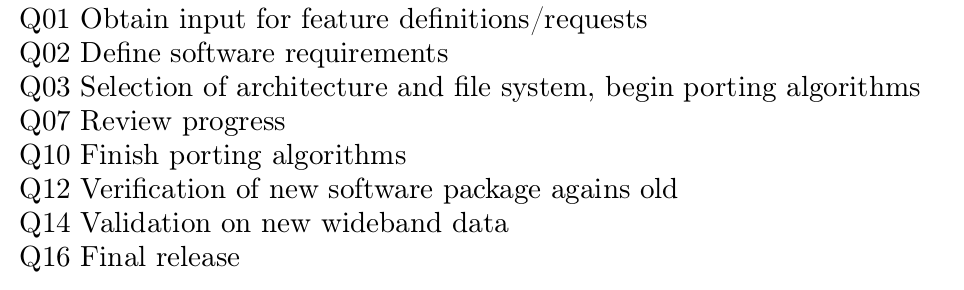
\includegraphics[width=0.70\textwidth]{nuHOPStimeline}}}
  \caption[Proposed Quarterly Plan]{This snippet from the proposal shows the original quarterly plan of develop for the ``new'' HOPS project.  Notionally the project kicked-off Oct 1, 2019, so Q1 is Oct--Jan of that year.  Notionally, then the final quarter, Q16 is July--Sep of 2023.}
\label{fig:prop-quarterly}
\end{figure}

After the proposal was accepted, the work was waterfalled into a Gantt format (see Fig.~\ref{fig:ganttcrap}) which is useful to establish that the tasks proposed are plausible for the time allowed.  The project shall be using an agile development methodology which does not lend itself to a waterfall diagram.
\begin{figure}[!h]
  \captionsetup{width=0.7\linewidth}
  \center{\fbox{%
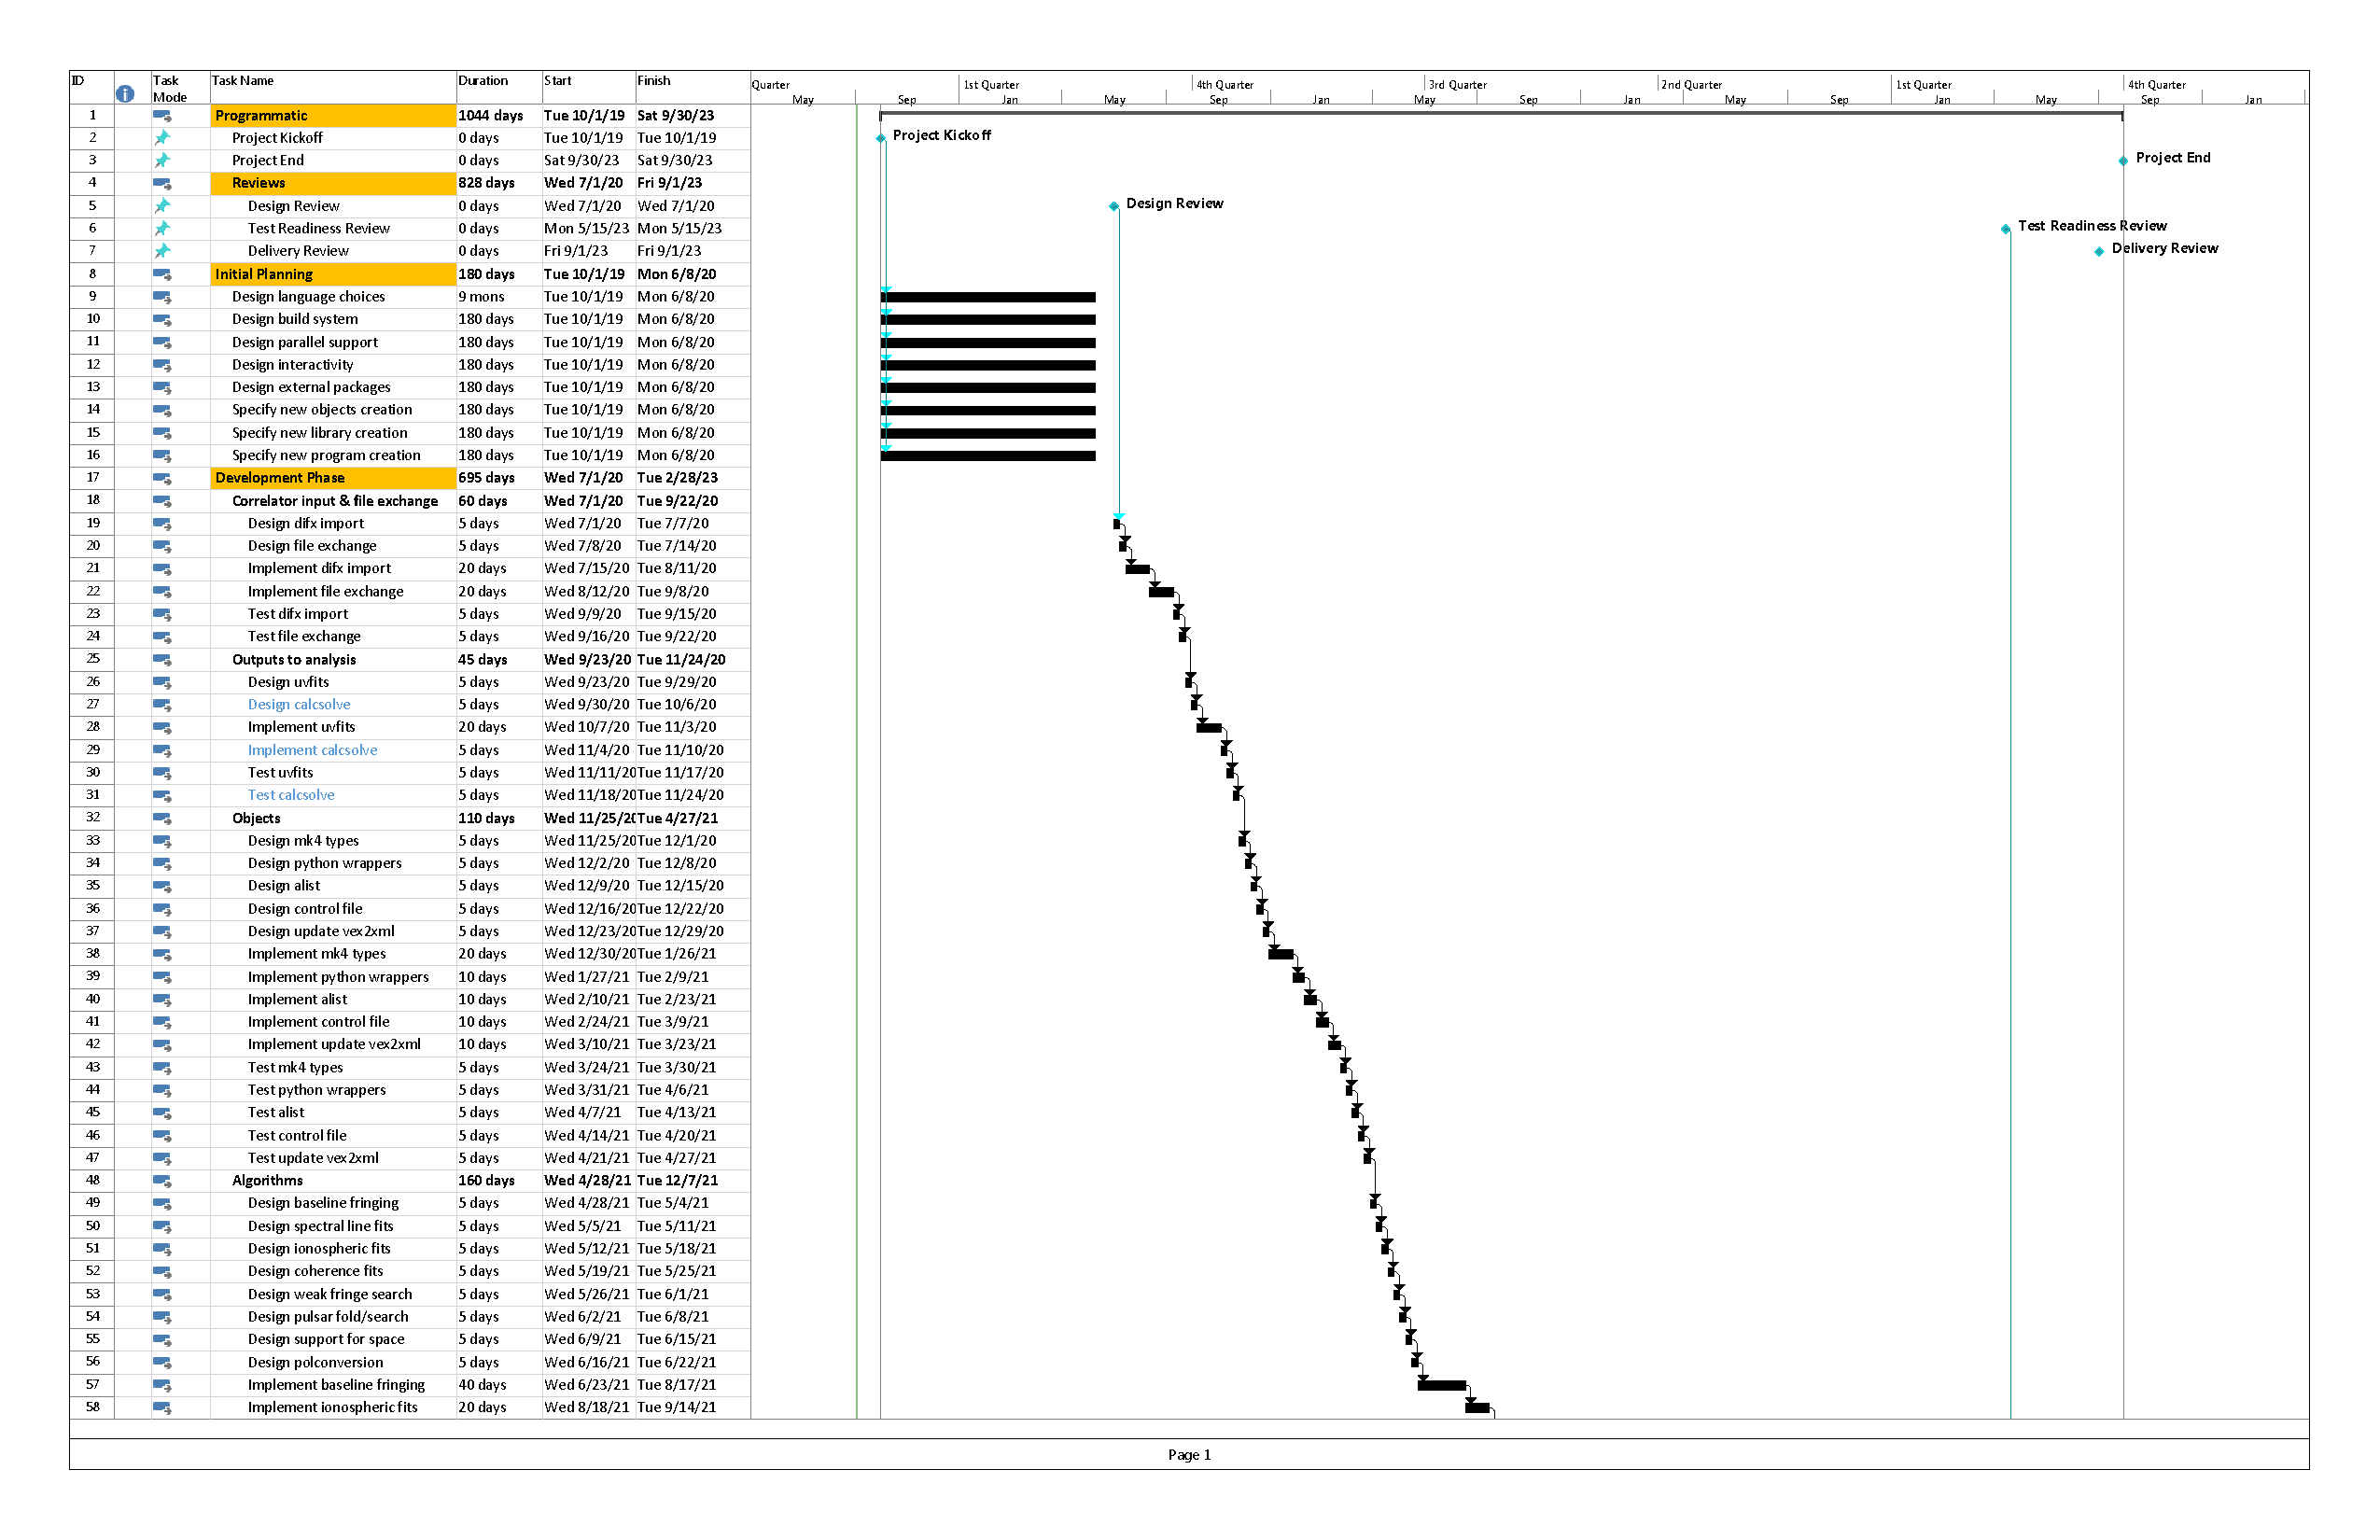
\includegraphics[width=0.40\textwidth]{MSRI-task-origv3-1}
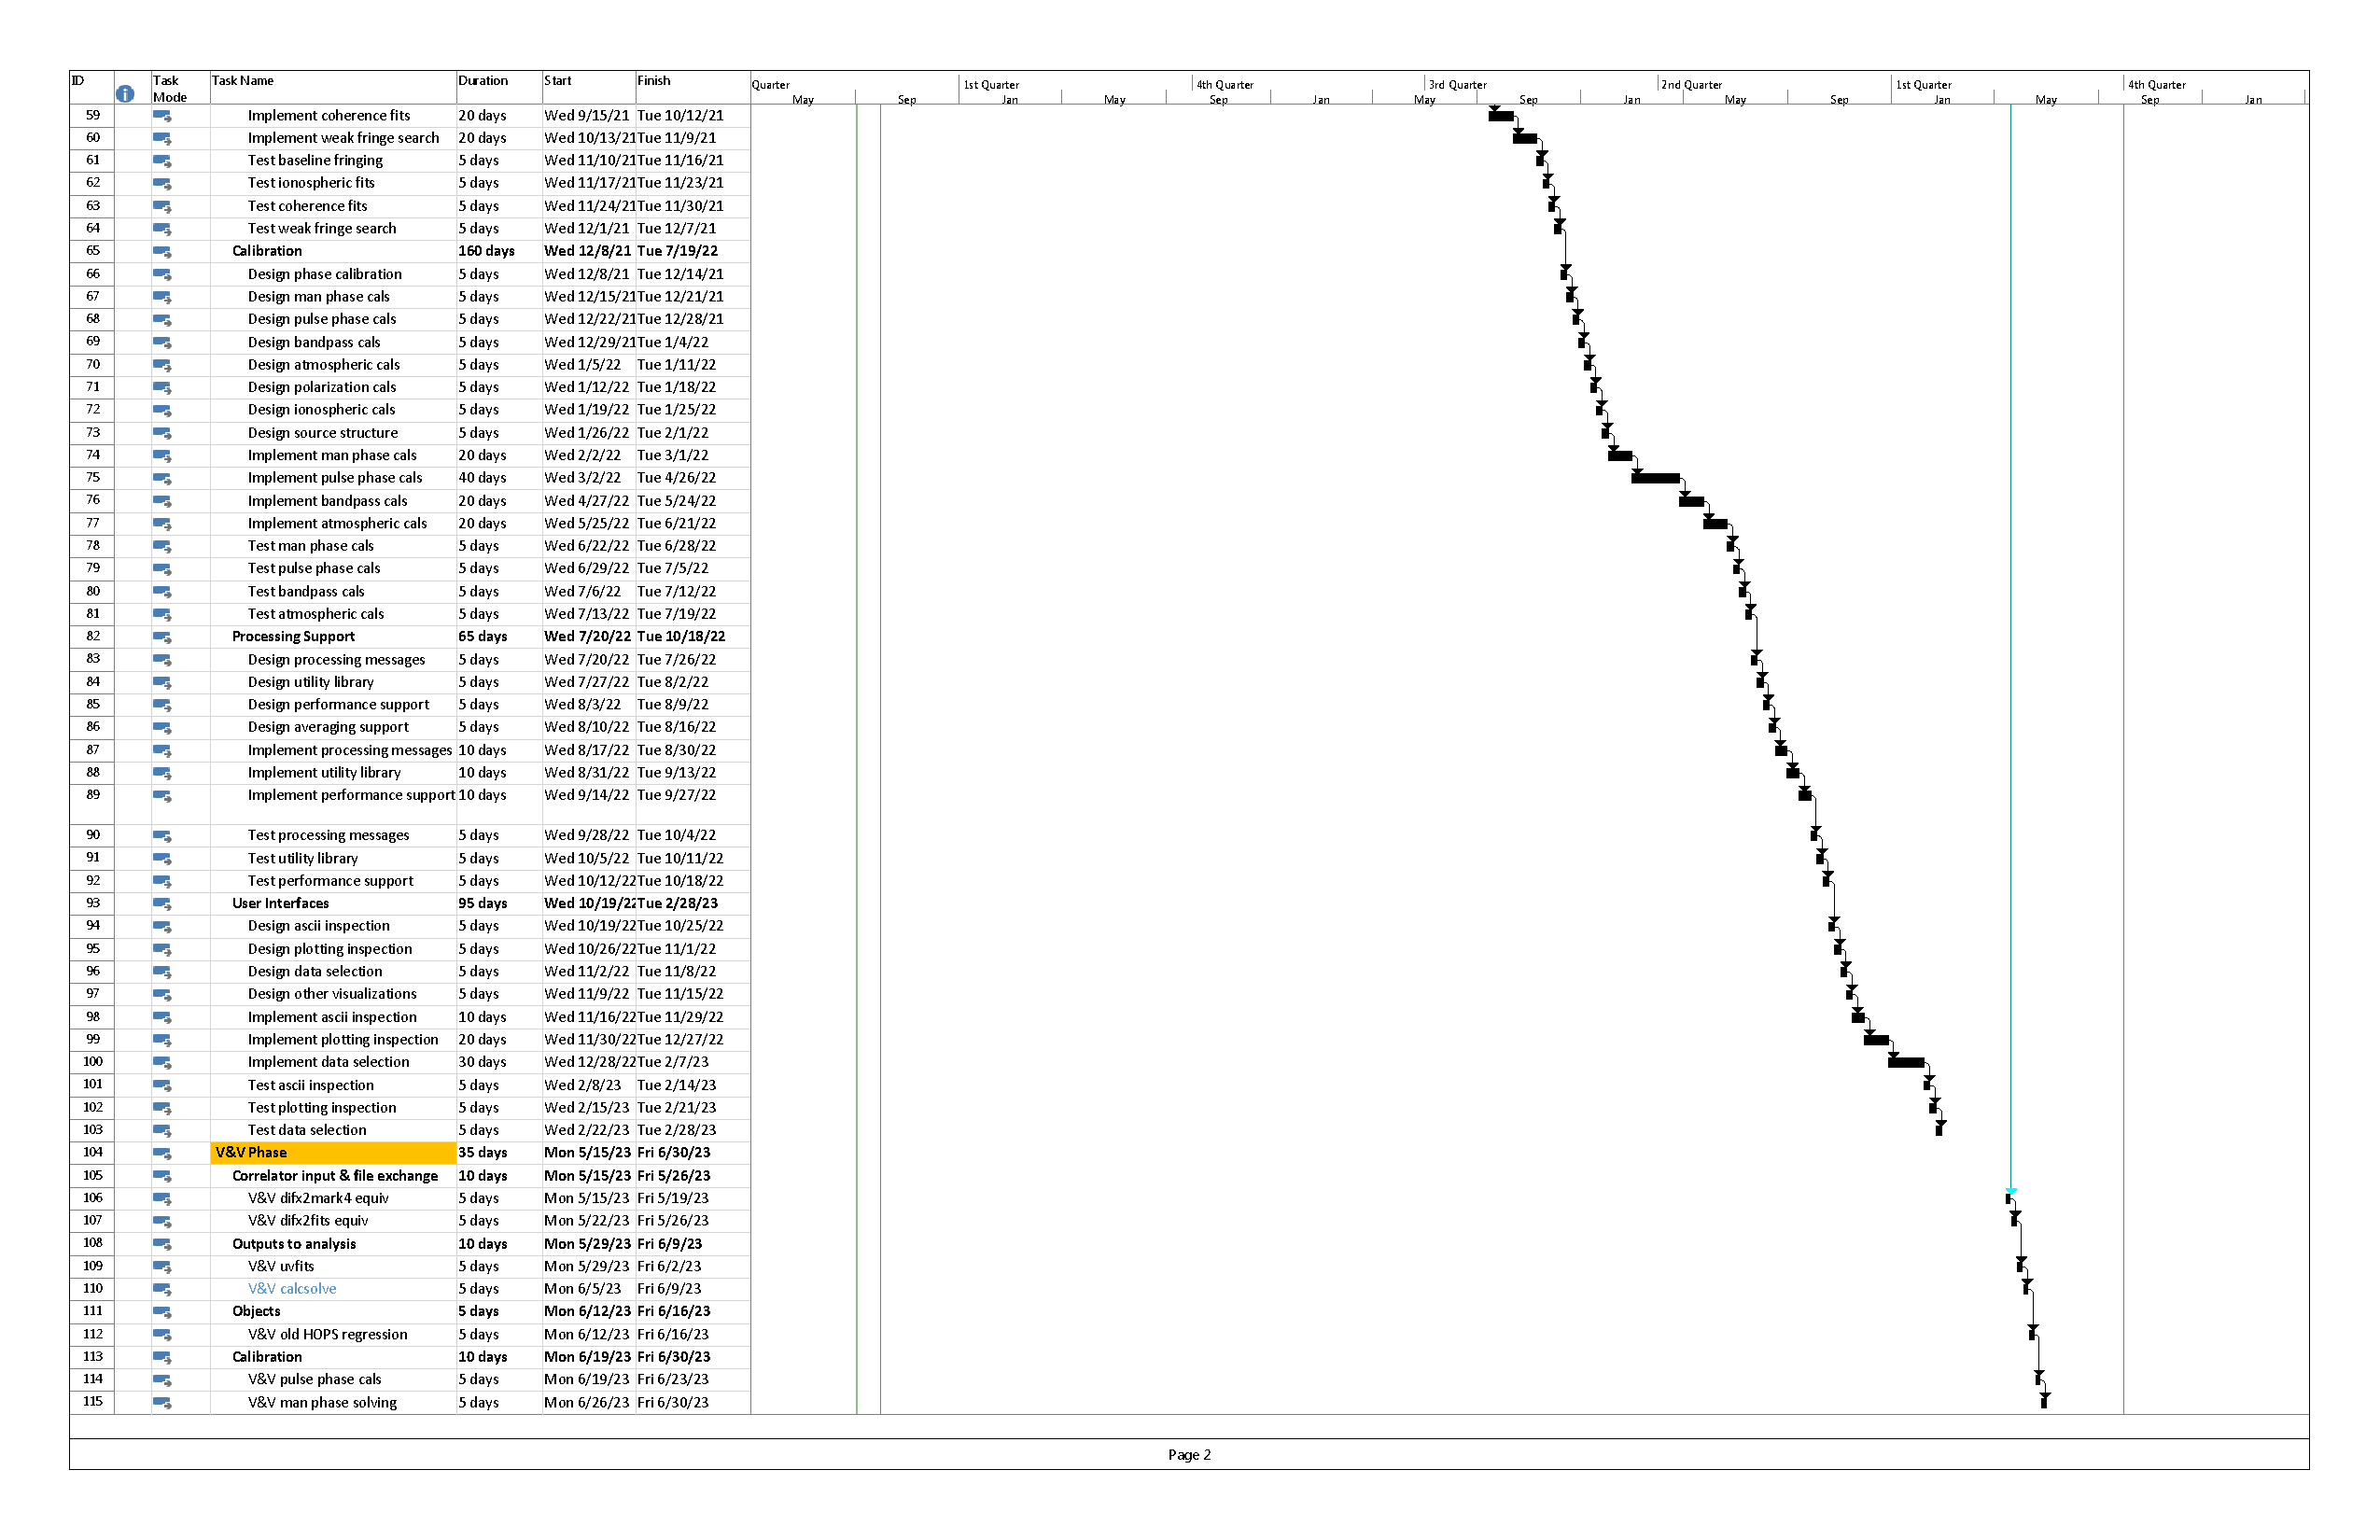
\includegraphics[width=0.40\textwidth]{MSRI-task-origv3-2} }}
\caption[Initial Gantt Timeline]{%
At the outset, a waterfalled Gantt-formulation of the work was
made to show that the 4-year timeline and estimated work effort
was consistent. The left panel corresponds to Q01--Q08, and the
right panel corresponds to Q09--Q16.}
\label{fig:ganttcrap}
\end{figure}

The COVID-19 pandemic slowed the initial stages of the project, especially the hiring of software developers (Hoak \& Pfieffer).  Nonetheless, a requirements review was held with EHT stakeholders in February 2021 (Q6 of the proposed schedule).

\subsubsection{Phase Plan}

\FIX[Define major milestones and achievement criteria; this section relies on the Detailed Timeline?]

\subsubsection{Iteration Objectives}

\FIX[Do we plan to iterate? If so:]

Iterations of the HOPS4 project will occur at points where various functionality is established. For example, the initial \texttt{fourfit} application will likely be imported from the existing HOPS3 libraries with minor reorganization; in this iteration, \texttt{fourfit} will run in HOPS4, but have the same underlying code and functionality as HOPS3. In a later release, the fourfit modules will be refactored to enable modularization of the application and extension to meet the \ac{ngEHT} requirements on stations, baselines, bands, etc.

\FIX[specify iterations? new data containers; refactoring of alist, aedit; no more PGPLOT; etc. Are iterations internal?]

\subsubsection{Releases}

\FIX[Do we plan to have releases? If so:]

HOPS4 will have a series of demo and beta releases prior to the final release, to allow stakeholders to test particular applications of the software. As a part of the agile development process, the schedule of releases is notional

\FIX[specify releases? new control file syntax, python interfaces, etc]

\subsubsection{Project Resourcing}

The current staff for the HOPS4 project (Barrett, Crew, Hoak, Pfieffer) have extensive software development experience across multiple languages (C/C++, Python, Perl, etc).  Crew and Barrett have used and maintained the exisiting HOPS package for years, and are familiar with its use-cases, functions and dependencies.

\subsection{Project Monitoring and Control}

\subsubsection{Requirements Management}

Requirements for the HOPS4 project are defined in the Requirements document. Changes to the requirements will be escalated to the project management, who will decide whether to alter the scope in order to preserve target completion dates.

\FIX[Mention requirements that may be de-scoped?]

\subsubsection{Schedule and Budget Control}

Expenses are primarily salary, which is fixed.

Schedule is monitored using the Detailed Timeline, which includes the expected duration and date for each milestone. Changes to the schedule will be escalated to the project management, who will decide whether to alter the scope in order to preserve target completion dates.

\subsubsection{Quality Control}

The HOPS4 project will have a extensive suite of tests, designed to verify the functionality of the software across the defined requirements. Existing functionality (from HOPS3) will be verified with automated check scripts using captured data.  New functions, modules and libraries will be delivered with unit tests to verify their functionality across different platforms and environments.  Furthermore, the project will use a continuous integration server to verify that the software compiles successfully after new commits, and profiling tools will be used to measure and monitor software performance (memory usage, CPU time, etc).  The details of the HOPS4 tests are described in the Coverage \& Testing document.

Defects (for example poor performance of a particular module in a particular environment) will be tracked through issues in the project git repository. 


\subsubsection{Reporting and Measurement}

The suite of HOPS4 tests shall be designed such that their output can be captured in reports. These reports will be organized to demonstrate progress towards the project requirements (\FIX[graphical trends?]). 

\subsubsection{Risk Management}

Risks are tracked by the \ac{ngEHT} management. Risks can be raised by any team member, are discussed internally at weekly meetings, and are reported and updated to \ac{ngEHT} management at monthly meetings. Risks for the HOPS4 project are primarily schedule risks, \eg that significant developer time may be needed to mitigate them.

Currently, only two risks are tracked:

\begin{itemize}

\item \textbf{Undiscovered bug in commit} A software deficiency or bug is discovered late in the project lifecycle which requires significant developer resources to correct. This may result in de-scoped requirments to remain on schedule. Continuous testing \& profiling is used to mitigate the likelihood of a serious deficiency.

\item \textbf{Incomplete ngEHT requirements} A critical use case is specified late in the project lifecycle, which requires significant developer time to extend or adapt the code. Modular code design will be used so that extensions \& restructuring are mitigated. 

\end{itemize}


\subsubsection{Configuration Management}

We use an MIT-hosted Gitlab Enterprise for tracking changes and issues.  Integration and regression tests are run on a daily or per-commit schedule.

\FIX[Do we need to mention backups?]

%
% eof
%

% Risk Management
% Measures of success
% Product Assurance
% Project closeout
%\input{}

\pagebreak
%%
%  original proposed schedule, for reference
%
\section{Proposed Plan}
\label{sec:prop-plan}

For reference, the ``new'' HOPS project was proposed with
a 4-year timeline with funds adequate to support one FTE.
The 

%
% eof
%


% if skipappendix-is-true then (nothing) else typeset Appendices
\ifthenelse{\boolean{skipappendix}}{}{%

\pagebreak
\appendix
\section{Acronyms, Commands and Glossary}
%
% \section{Acronyms, Commands and Glossary}
%
% \acro{acronym}[short name]{full name / description}
% \ac{acronym} is the usual usage in text that defines (and gives short name)
% \acs{acronym} gives just the short name
% \acf{acronym} gives just the full name
% \acsu{acronym} gives the short name and marks it used
% \a..p{acronum} makes it plural
%
% the optional short name can include math as the acronym key cannot
% there are a zillion other options, see https://ctan.org/pkg/acronym
%
\begin{acronym}
% A---------------------------------------------------------------
\acro{A-list}{a one line description of baseline fringes used by \ac{HOPS}}
\acro{adump}{a program that dumps columns from \ac{A-list} scan data}
\acro{alist}{a program for creating a file of \ac{A-list} scan data}
\acro{aedit}{a program for editing a file of \ac{A-list} scan data}
\acro{average}{a program that calculates averages on \ac{A-list} scan data}
\acro{AIPS}{Astronomical Image Processing System}
\acro{ALMA}{Atacama Large Millimeter/Submillimeter Array}
\acro{AMP}{short for ``amplitude'' the correlation coefficient}
\acro{AP}{Acquision Period which refers to a period of time over which the
    correlator integrates the input (noisy) data to produce a usable output.
    Terms such as \acs{dump} or ``integration'' are also sometimes used,
    but both can be ambiguous.}
\acro{awk}{A programmable language for parsing line and field oriented input.
    The program was part of the original \acs{UNIX} product, and is named for
    its three authors,  Alfred Aho, Peter Weinberger, and Brian Kernighan}
% B---------------------------------------------------------------
\acro{bigendian}{refers to a computer hardware architecture where the
    most significant
    bits of a larger storage object (bytes, words\ldots) are serialized first.}
\acro{bit}{a 0 or 1}
\acro{byte}{a unit of storage corresponding to 8 bits}
% C---------------------------------------------------------------
\acro{C}{The ``C'' programming language, created to make \ac{UNIX} portable}
\acro{C++}{The C++ programming language, an object-oriented
    successor to \ac{C}}
\acro{C/C++}{Refers to code that may be either \acs{C}, \acs{C++} or a mix of
    the two ``dialects''.  The two compliers currently in use in the project,
    \acs{GCC} and \acs{Clang} manage both dialects.}
\acro{CASA}{Common Astronomy Software Applications}
\acro{channel}{an ambigous term which refers either to a spectral channel,
    \ie~frequency point of an \acsu{FFT} or to a sub-band of a
    larger receiver band.}
\acro{cofit}{a \ac{HOPS} tool to assess atmospheric coherence in terms of
    \ac{SNR} and \ac{AMP} variation with integration interval}
\acro{CorAsc2}{Correlator to Ascii (2nd version)}
\acro{cover}{a coverage test exercises all logic branches of some code module}
% D---------------------------------------------------------------
\acro{DFT}{Discrete Fourier Transform}
\acro{DR}{Delay Rate, the fringe parameter concerning
    the change of delay with time}
\acro{DiFX}{the ``distributed'' \ac{FX} correlator}
\acro{difx2mark4}{a program (part of \ac{DiFX}) to convert \ac{SWIN}
    format correlation products into the ``Mark4'' (or \acs{Mk4})
    data files used by \ac{HOPS}}
\acro{dump}{a term used with hardware correlators to refer to a time
    integration performed by hardware/firmware circuitry.  The dumped
    data may then be further integrated in software.}
% E---------------------------------------------------------------
\acro{EHT}{the Event Horizon Telescope}
\acro{EHTC}{the Event Horizon Telescope Collaboration, which usually
refers to the organization that operates the \ac{EHT}}
% F---------------------------------------------------------------
\acro{FFT}{Fast Fourier Transform}
\acro{FFTW3}{Fastest Fourier Transform in the West, version 3}
\acro{Fortran}{a FORmula TRANslation language, in common use prior to \ac{C}}
\acro{FX}{a general term for correlation that does the cross-correlation
    after first transforming to frequency space}
\acro{FITS}{Flexible Image Transport System, now referring to a
    general digital data format}
\acro{FITS-IDI}{A dialect of \ac{FITS}
    designed for the interchange of data for interferometry}
\acro{flag}{A term commonly used in radio astronomy to mark bad data
    for exclusion from further analysis.}
\acro{fourfit}{the main fringe-finding command in \ac{HOPS}}
\acro{fringex}{an \ac{HOPS} tool to explore the fringe} 
\acro{fourmer}{a program that combines data from two sub-bands into
    a larger common band}
% G---------------------------------------------------------------
\acro{ghostscript}{Ghostscript, the GNU \acs{PostScript} emulator}
\acro{Gbps}{refers to data recording rate, usually.  8 Gbps is 1 GB/s
    or one billion characters (of ASCII) per second.  Usually there
    are (packet) overheads in the actual recording so the write or
    playback speed may be somethings slightly or grossly different.
    The \ac{HOPS} era started with kbps worked through Mbps and ended
    with Gbps.  Tbps will probably be with us in another decade.}
\acro{GHz}{one billion Hz}
\acro{GNU}{GNU is Not Unix (a software project launched by
    Richard Stallman in the 80's)}
\acro{GNU/Linux}{a family of operating systems using Linus' kernel and
    GNU's software packages}
\acro{grep}{global regular expression parser, a name for a collection of
    tools that perform regular expression parsing of input data strings.}
\acro{GS}{short for \ac{ghostscript}}
\acro{GSL}{\acs{GNU} Science Library, a library of functionality for
    science applications.}
\acro{GUI}{Graphical User Interface}
% H---------------------------------------------------------------
\acro{HDF5}{Hierarchical Data Format, version 5.\protect\footnote{Why would you
    \textit{want} to use anything that took 5 versions to get right?}}
\acro{HOPS}{Haystack Observatory Postprocessing System}
\acro{Hz}{A frequency unit named for Heinrich Hertz.
    A frequency of one Hz is one oscillation per second.}
% I---------------------------------------------------------------
\acro{i/o}{short for input/output referring to the fact that programs are
    written to act on something and provide something}
\acro{IPP}{Intel Performance Primitives is a library of functionality
    optimized for use with the Intel processor family}
% J---------------------------------------------------------------
\acro{JIVE}{now just a name for an organization, it is still an
    Institution for VLBI in Europe, just not a Joint one}
% L---------------------------------------------------------------
\acro{Linux}{a family of operating systems built around Linus Torval's version
    of the UNIX kernel}
\acro{littleendian}{refers to a computer hardware architecture where the
    least significant
    bits of a larger storage object (bytes, words\ldots) are serialized first.}
\acro{LSF}{Least Squares Fit}
% M---------------------------------------------------------------
\acro{MBD}{Multi-Band Delay, the delay parameter referring to the change of
    phase with frequency in a multi-channel (sub-band) system.}
\acro{Mk4}{The fourth in a series of \ac{VLBI} hardware correlators.  The
    Mark4 replaced the Mark3 near the beginning of the millenium, and was
    finally put to rest by \ac{DiFX} in the mid 2010's}
\acro{m4py}{a shallow \acs{Python} wrapper which provides access to
    \acs{Mk4} data files and types}
\acro{MS}{Measurement Set, a formal specification for data to be analyzed
    with reference to a Measurement Equation}
\acro{MSRI}{Mid-scale Research Initiative}
% N---------------------------------------------------------------
\acro{NSF}{National Science Foundation}
\acro{ngEHT}{next-generation \acs{EHT}}
% O---------------------------------------------------------------
\acro{ovex}{an ``observer'' dialect of \acs{VEX}}
\acro{OpenMPI}{Open MPI Project is an open source Message Passing Interface
    implementation}
% P---------------------------------------------------------------
\acro{PDF}{Portable Document Format (developed by Adobe) as a successor
    to \ac{PostScript}}
\acro{PGPLOT}{a ``pretty good'' plotting package developed and maintained
    by Tim Pearson at Caltech.  He's retired now, so it is stuck at verion
    5.2.2, (released Feb 2001)}
\acro{PostScript}{a printer page description language developed by Adobe.
    \ac{fourfit} plots are currently generated in \ac{PostScript} and
    often converted to \acs{PDF}}
\acro{PERL}{Practical Extraction and Reporting Language created by Larry Wall}
\acro{PS}{short for \ac{PostScript}}
\acro{Python}{a programming language named in honor of Monty Python's Flying
    Circus}
% R---------------------------------------------------------------
\acro{RFI}{Radio Frequency Interference which is what you have when your
    receiver picks up signals you do not want}
% S---------------------------------------------------------------
\acro{SBD}{Single Band Delay, the delay parameter referring to the time
    offset between two signals being correlated}
\acro{search}{this is a tool that searches in delay/delay-rate space to
    allow visualization of a fringe peak and to aid in establishing the
    validity of more marginal-\acs{SNR} cases}
\acro{sed}{is a stream editor, that ingests line-oriented data and performs
    programmatic operations on it prior to output}
\acro{SFXC}{\acs{JIVE}'s software \ac{FX}-kind correlator}
\acro{SNR}{Signal to Noise Ratio}
\acro{SWIN}{the output format used by the \ac{DiFX} correlator}
\acro{MHO}{MIT Haystack Observatory Postprocessing System}
% T---------------------------------------------------------------
\acro{TEC}{Total Electron Content, refering to the column density of
    electrons in the line of sight through the ionosphere.  Conventionally
    one TEC Unit is \protect{$10^{16}$ electrons / m$^2$}}
% U---------------------------------------------------------------
\acro{unit}{a unit test is a short test used to validate a small part of
    some larger code module}
\acro{Unicode}{here, a general reference to a collection of methods for
    representing printable characters beyond ASCII.  The painful
    \ac{Python} 2 to 3 transition was driven by a need to more correctly
    handle strings of Unicode character representations.}
\acro{UNIX}{the name of a family of operating systems
    (born in the 70's at Bell Laboratories)}
% V---------------------------------------------------------------
\acro{VEX}{\acs{VLBI} EXperiment (file), a means of fully describing
    a planned \acs{VLBI} experiment or observation}
\acro{VEX2XML}{a program that converts \acs{VEX} files into an easily
    parsed \acs{XML} represention}
\acro{VGOS}{\acs{VLBI} Global Observing System;
    was called \acs{VLBI}2010 until the mid 2010's}
\acro{VLBI}{Very Long Baseline Interferometry}
% W---------------------------------------------------------------
\acro{Whitneys}{correlation amplitudes are normally expressed between 0 and 1,
    but in our work they are usually small and in \ac{HOPS} traditionally
    multiplied by ten thousand, in which case, the unit of correlation amplitude
    is ``Whitneys'' after Alan Whitney who may be commended or blamed for the
    usage.}
\acro{word}{an architecture-dependent unit of storage---these days, most of
    our processors use 8-\acs{byte} words}
% X---------------------------------------------------------------
\acro{XF}{a general term for correlation that does the cross-correlation
    first, and then transforms the result to frequency space}
\acro{XML}{eXtensible Markup Language}
% Z---------------------------------------------------------------
\acro{zero-pad}{the practice of extending time or frequency sequences with
    some number of zeroes which, for \ac{FFT}s has the effect of smoothing
    in the other domain}
\end{acronym} 
%
% eof
%


}

\pagebreak
\addtocounter{section}{1}
\renewcommand{\refname}{\thesection. References}
\addcontentsline{toc}{section}{\thesection. References}
\bibstyle{plainurl}
\printbibliography
\label{sec:references}

\label{page:LastPage}
\end{document}
